\chapter{Implementation}
\label{chapter:implementation}
\section{Option Pricing}
\label{section:Option Pricing}
The theoretical models presented in Chapter \ref{chapter:background} attempt to model the movements of real-world stock prices. With the predictions obtained, we should be able to better replicate real option prices than if we assumed a simple constant volatility.

Currently, the two most used methods to computationally price options are known as \emph{finite differences}~\cite{Hull} and \emph{Monte Carlo}~\cite{Glasserman}.

Finite differences is an extremely fast procedure when used to price either European or American-type options, making it very appealing in these circumstances. However, when used to price other option types whose value depends on the stock prices until maturity (e.g. Asian options), the algorithm becomes very slow, rendering it almost useless.
The implementation of both Heston and SABR models (presented before) using finite differences can be found in deGraaf~\cite{deGraaf}.


With the Monte Carlo method, the algorithm simulates a very large number of stock price paths (e.g. 100,000 simulations), under the selected model's assumptions. The option payoff is then calculated for each of these paths and averaged, providing a fair estimate of the option's value. This algorithm can also be easily adapted to price exotic options, making it very attractive in such cases.
In the past, simulating all the stock paths took prohibitively long computation times and this method was often discarded for this reason. However, with the recent advancements in computer hardware and new algorithmic developments, such as GPU implementation, this method has become quite popular.
For these reasons, the Monte Carlo method will be used for the validation of the models presented before.


\subsection{Simulating stock prices}
\label{subsection:Simulating stock prices}
As stated, to implement the Monte Carlo algorithm one needs to simulate stock price paths. However, by analyzing eq.\eqref{GBM}, we can see that the stock prices depend on a Brownian motion process (also known as a Wiener process) which, due to its self-similarity, is not differentiable~\cite{Mikosch}. It follows that stock price paths can never be exactly simulated.

\subsubsection{Euler–Maruyama discretization}
\hl{put this in background section?} Though exact simulation is impossible, we can approximate the movement of stock price paths using the Euler–Maruyama discretization, which can be applied to stochastic differential equations of the type
\begin{equation}\label{SDE}
dX(t)=a(X(t))dt+b(X(t))dW(t),
\end{equation}
\noindent where $a(X)$ and $b(X)$ are some given functions and $\{W(t),\ t>0\}$ defines a one-dimensional Brownian motion process.
To apply this discretization, we begin by partitioning the simulation interval $[0,T]$ into $N$ subintervals of width $\Delta t=T/N$ and then recursively define
\begin{equation}
X_{n+1}=X_n+a(X_n)\Delta t+b(X_n)\Delta W_n,
\end{equation}
\noindent for $n=1,\ldots,N$ where $\Delta W_n=W_{t+\Delta t}-W_{t}$.
Using the known properties of Brownian motion processes, we can produce $\Delta W_n\sim \sqrt{\Delta t}Z$, where $Z\sim N(0,1)$ defines a standard normal distribution.

Applying this discretization to the Geometric Brownian motion followed by stock price paths (as seen in eq.\eqref{GBM}), we arrive at
\begin{equation}
S(t+\Delta t)=S(t)+rS(t)\Delta t+\sigma S(t)\sqrt{\Delta t}Z.
\end{equation}

Due to its simplicity, the Euler–Maruyama discretization method is the most common in the simulation of stock price paths.


\subsubsection{Milstein Discretization}
For stochastic volatility models, such as Heston and SABR, where the volatility itself follows a stochastic differential equation (as in eq.\eqref{SDE}), the Euler–Maruyama discretization may not be sufficiently accurate. In these cases, we can easily apply the more precise Milstein method~\cite{Milstein}, defined as
\begin{equation}
X_{n+1}=X_n+a(X_n)\Delta t+b(X_n)\Delta W_n+\frac{1}{2}b(X_n)b'(X_n)((\Delta W_n)^2-\Delta t),
\end{equation}
\noindent where $b'(X_n)$ denotes the derivative of $b(X_n)$ w.r.t. $X_n$. Note that when $b'(X_n)=0$, the Milstein method collapses to the simpler Euler–Maruyama discretization.

Applying this discretization to the Heston model, we arrive at
\begin{equation}
S(t+\Delta t)=S(t)+rS(t)\Delta t+S(t)\sqrt{\nu(t)}\sqrt{\Delta t}Z_1+\frac{1}{2}\nu(t)S(t)\Delta t(Z_1^2-1),
\end{equation}
\begin{equation}
\nu(t+\Delta t)=\nu(t)+\kappa(\overline{\nu}-\nu(t))\Delta t+\eta\sqrt{\nu(t)\Delta t}Z_2+\frac{\eta^2}{4}\Delta t(Z_2^2-1),
\end{equation}
\noindent where $Z_1$ and $Z_2$ are two normal random variables with a correlation of $\rho$.


Applying the Milstein discretization to the SABR model results in
\begin{equation}
F(t+\Delta t)=F(t)+\sigma(t)F^\beta(t)\sqrt{\Delta t}Z_1+\frac{\beta}{2}\sigma^2(t)F^{2\beta-1}(t)\Delta t(Z_1^2-1),
\end{equation}
\begin{equation}
\sigma(t+\Delta t)=\sigma(t)+\nu\sigma(t)\sqrt{\Delta t}Z_2+\frac{\nu^2}{2}\sigma(t)\Delta t(Z_2^2-1),
\end{equation}
\noindent where again $Z_1$ and $Z_2$ are two normal random variables with a correlation of $\rho$.

To generate two correlated normal variables $Z_1$ and $Z_2$, we can extract $Z_1$ from a standard normal distribution and produce $Z_2$ from
\begin{equation}\label{normcorr}
Z_2=\rho Z_1+\sqrt{1-\rho^2}W,
\end{equation}
\noindent where $W$ is a normal random variable, uncorrelated with $Z_1$.

Because it is more precise, the Milstein method will be used in the implementation of both Heston and SABR stochastic volatility models. The simpler Euler–Maruyama discretization will be assumed for Dupire's local volatility as well as for constant volatility.


\subsection{Pricing options from simulations}
\hl{this should come before the discretization methods?}
To price options, we generate $M$ paths by recursively calculating $S_i(t)$ (or $F_i(t)$ in the case of SABR), for $i=1,\ldots,M$, using either discretization method. When the stock price at the maturity is obtained (i.e. $S_i(T)$ or, in the case of SABR, $F_i(T)=S_i(T)$), the option payoff for each path is calculated from eq.\eqref{callput}. Discounting these values to the present, we obtain the (call) option value
\begin{equation}
C(K,T)=e^{-rT}\frac{1}{M}\sum_{i=1}^M\max\left(S_i(T)-K,0\right).
\end{equation}

It is important to note that, the smaller our subintervals $\Delta t$ are, the better our discretization methods replicate real Brownian motion processes. However, by decreasing $\Delta t$ we increase the number of intervals and with it the number of calculations needed to obtain each $S_i(T)$. The compromise between computation time and precision must be handled appropriately.
 \hl{put some image here to exemplify the different time steps dt}



\iffalse
depend on a Brownian motion process, it follows that it is not differentiable. For this reason, it's impossible to exactly simulate such a process. An approximation is possible, however, using discrete jumps of length $\Delta t$ and using the Brownian motion property $W(t)\sim \sqrt{t}N(0,1)$~\cite{Mikosch}, with $N(0,1)$ being a normal distribution with 0 expected value and 1 variance.
We can then simply discretize eq. \eqref{BS} into
\begin{equation}
S(t+\Delta t)=S(t)+rS(t)\Delta t+\sqrt{\Delta t}\sigma S(t)N(0,1),
\end{equation}
\noindent where $\Delta t$ corresponds to a given time step. An example of this discretization is illustrated in \autoref{fig:GBM} with the realization of three sample paths.

\begin{figure}[H]
    \centering
      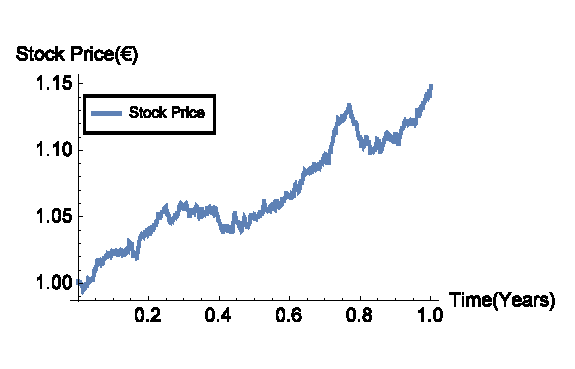
\includegraphics[width=0.9\columnwidth]{GBM.eps}
      \caption{Example of three GBM processes, using the parameters $r=\SI{0.06}{\per\year}$, $\sigma=0.05$, $S(0)=\SI{1}[\EUR]{}$ and time steps $\Delta t=10^{-3}\SI{}{\year}$.}\label{fig:GBM}
    \end{figure}
    
By simulating a large number of paths, some underlying tendencies might become apparent, which will prove useful in option pricing.


 American options, however, pose a much greater challenge.  Unlike European options, no analytic pricing model currently exists for this type of derivatives. Several numerical models have been proposed in the past in an attempt to solve this problem~\cite{Wilmott1,Hull}, such as the Longstaff-Schwartz algorithm~\citep{Longstaff}, which we shall approach in later sections of the present thesis.
\fi 

 
 
 
\section{Model Calibration}
\label{section:Model Calibration}
Both SABR and Heston stochastic volatility models contain variables that need to be calibrated in order to appropriately replicate market option prices.

Calibrating the models' parameters means we find the optimal values for these parameters such that difference between the prices of market options and options priced under the models' assumptions is minimized. This difference should be measured with a cost function such as
\begin{equation}\label{cost}
\mathrm{Cost}(\theta)=\sum_{i=1}^n\sum_{j=1}^m\left(\frac{C_{\mathrm{model}}(\theta,T_i,K_j)-C_{\mathrm{market}}(T_i,K_j)}{C_{\mathrm{market}}(T_i,K_j)}\right)^2,
\end{equation}
\noindent where we denote $\theta$ as the model's parameter set, $C_{\mathrm{model}}(\cdot)$ and $C_{\mathrm{market}}(\cdot)$ the model and market option prices, respectively, for maturities $T_i,(i=1,\ldots,n)$ and strikes $K_j,(j=1,\ldots,m)$.


There are several possible algorithms to find the minimum value for the cost function shown in eq.\eqref{cost}. In general, most algorithms require some starting guess at the parameters' optimal values, $\theta'$, calculating then the cost function for these values, $\mathrm{Cost}(\theta')$. The initial values of the parameters are then slightly modified to some new values, $\theta^{*}$ and the cost function is recalculated, $\mathrm{Cost}(\theta^{*})$. If the error decreases after the modifications (i.e. $\mathrm{Cost}(\theta^{*})<\mathrm{Cost}(\theta')$), the new parameter values are assumed - otherwise they are discarded. This procedure is repeated until new changes in the parameters no longer decrease the cost function.
\hl{put "Algorithm" here?}

The main problem with this algorithm is the fact that the cost function may be nonlinear, meaning that it might present several local minima. This is problematic because the procedure will only progress in directions where the cost function gradient is negative. Thus, the optimizer will get stuck in these points and the global minimum will not be reached.
The minimum found by the algorithm should then be heavily dependent on our initial starting point, which is very undesirable.
Two possible workarounds exist around this problem: we could run the optimizer for several starting points until several (local) optima are found and choose the smallest one. We could also use stochastic optimization algorithms such as simulated annealing. With these, the optimizer usually follows the direction in which the cost function gradient is negative but there is a chance that a random new direction is chosen. Thus, if the optimizer gets stuck at a local minimum, it may be able to escape from it until, ideally, the global optimum is found.
Both workarounds will be studied in chapter \ref{chapter:results}.


The algorithm described before requires a very large number model pricer instances to be called. At each iteration, the pricer needs to run once for all maturities and strikes for which we have market data. This is problematic if the pricer takes too long to run and we should attempt to find ways to price options as fast as possible.

To price options, we could


One possible method to calibrate both Heston and SABR is to start with some initial guess at the parameters' values and run the Monte Carlo pricer, to obtain the option prices for the chosen parameters. We would then compare these model prices with those presented in the market and calculate the difference between them using some error measure, such as least-squares.

We would then iteratively modify the initial values of the parameters, and run the pricer again for each new value, accepting those that reduce the error function and rejecting the others.
Though this methodology appears simple, two potential problems can be pointed out. First, it should be noted that the Monte Carlo algorithm will take some time to run, and has to be executed once for each parameter change. A large number of steps may be required and the computation times add up, making the algorithm impractically slow. Secondly, the optimization algorithm may get stuck in some local minimum, not reaching the global optimum. Some stochastic optimization procedures (e.g. simulated annealing) may be used in this case, but the computation times would increase further.
This optimization algorithm can be sped up using GPU implementation, as has been done by Fernandez \textit{et al.}~\cite{Fernandez} for the Heston model.

\hl{globalsearch/multistart != stochastic optimization}


The main reason why Heston and SABR are so popular is the fact that both models have closed-form solutions (shown in eqs.\eqref{CH},\eqref{sabr} and \eqref{dynsabr}) that we can rapidly calculate. These solutions enable us to directly price the model options without the need to run the slow Monte Carlo pricer. The optimization algorithm should then converge quite fast. In these cases, we can use stochastic optimization algorithms to reach the global optimum, without much concern for the increased computation times.

Choosing the right stochastic optimization algorithm is important. Because our parameters are bounded,the chosen algorithm should accept parameter boundaries. It should also preferably be fast, though this is not the main concern in this work.

\subsection{Optimization algorithms}
\subsubsection{Global Search}

\subsubsection{Stochastic Optimization (Simulated Annealing)}

\subsection{Monte Carlo upgrades}

To calibrate SABR, we can either follow the Monte-Carlo approach and simulate a large number of paths, assuming stochastic volatility with some starting parameters and minimizing the difference between model-generated prices and real-world option prices, or we can use eq. xxx to obtain the implied volatility and minimize the market implied volatility.
